\chapter{Implementation}
This chapter will explain how the described concept has been implemented.
First an overview of the concept and then the main parts of the software in more
detail.
The trackable marker is attached to the ultrasound probe. The marker is
detectable by the tracking camera and enables the camera to determine the
position and orientation of the ultrasound probe. The probe on its own will
create an ultrasound image. Then the sampled ultrasound image and pose will be
post processed as a pair in the computer. In the software, depending on the
actual state of the surgery, the use of the two will be different.

\begin{figure}[H]
  \centering
 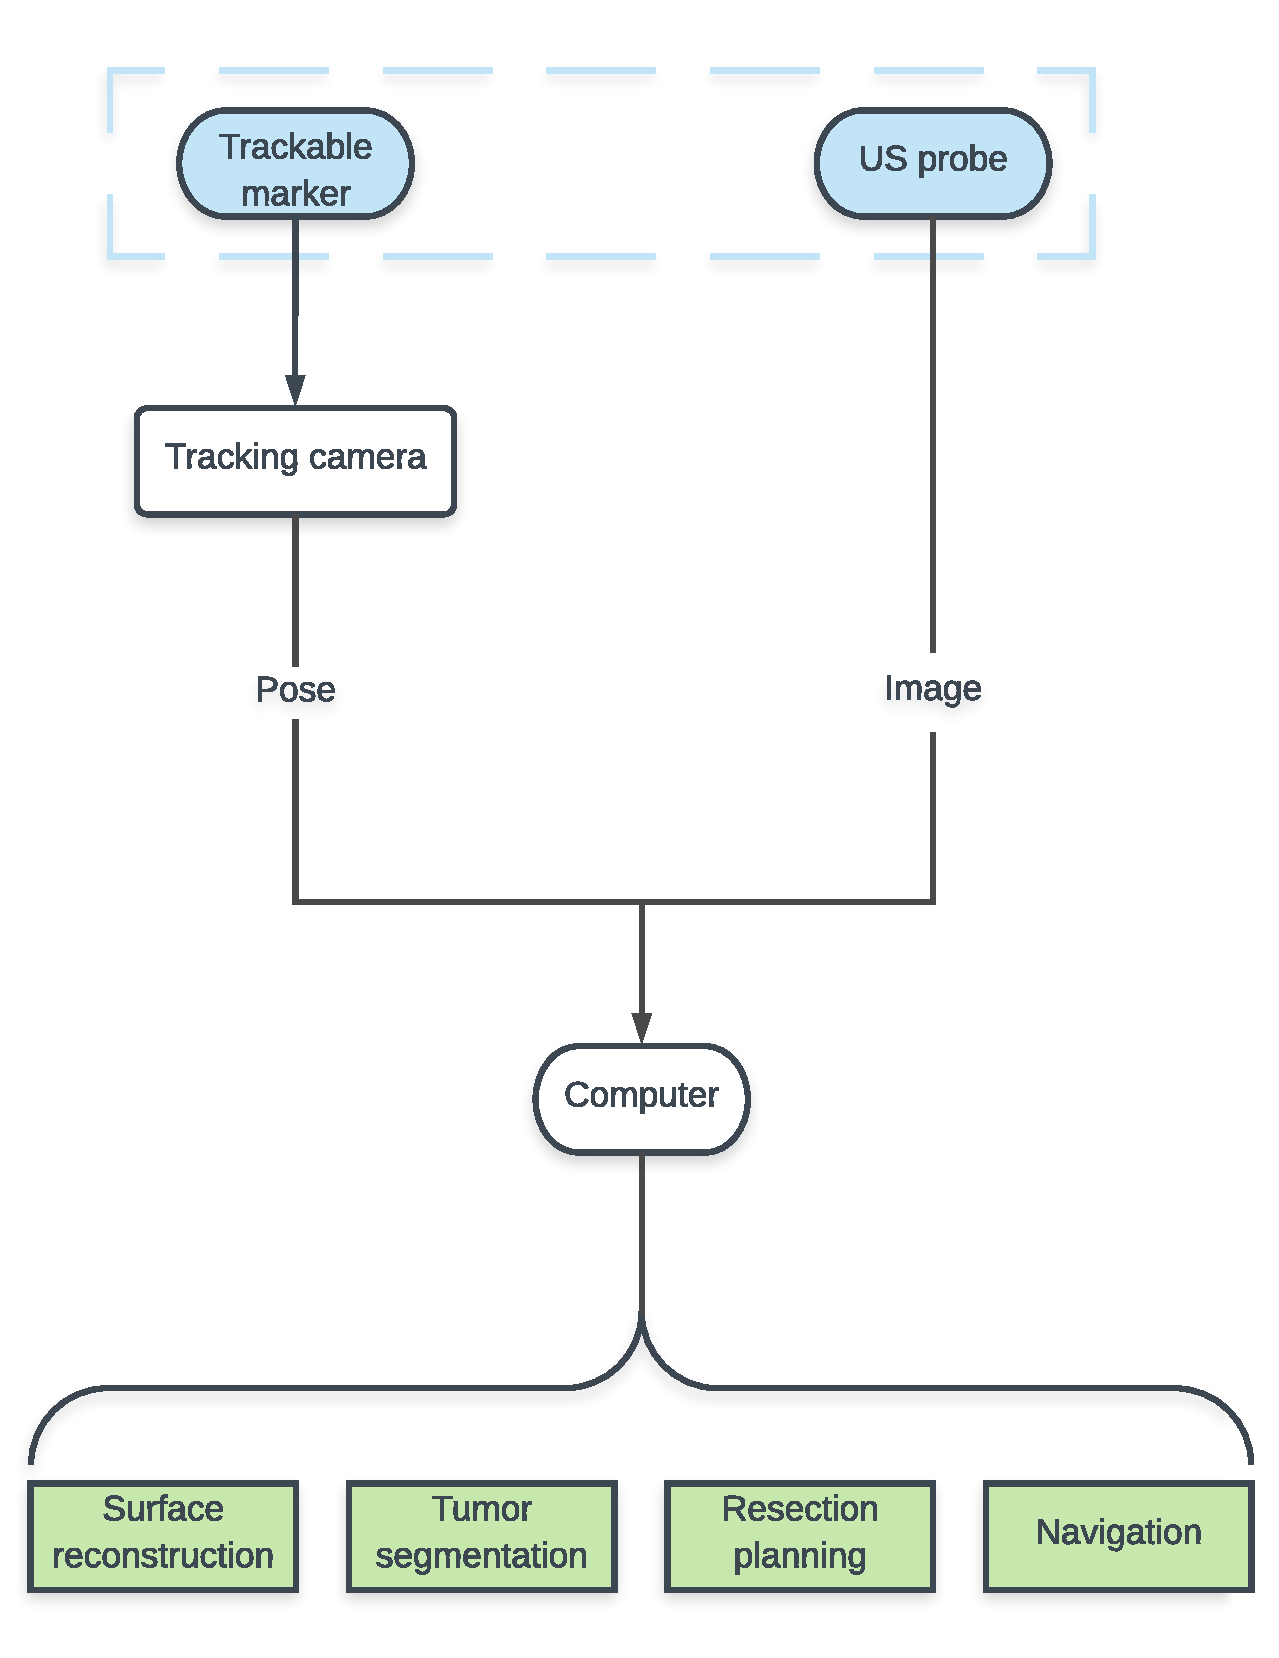
\includegraphics[width=0.65\textwidth]{FirstFlowChart}
  \caption{The way of the ultrasound image and the corresponding pose to the
    computer and later to the different parts in the software.}
  \label{fig:FirstFlowChart}
\end{figure}

\section{Surface Reconstruction}
While the surgeon is scanning the surface, the software in the background
filters out unusable positions. An image pose pair has to take two hurdles to
become accepted in the group of surface points. The image has to prove that it
arised from the liver surface and the position has to have a similar distance to
its neighbors as its neighbors to it. 
When enough points are sampled, the reconstruction of the surface will be
carried out.
\begin{figure}[H]
  \centering
 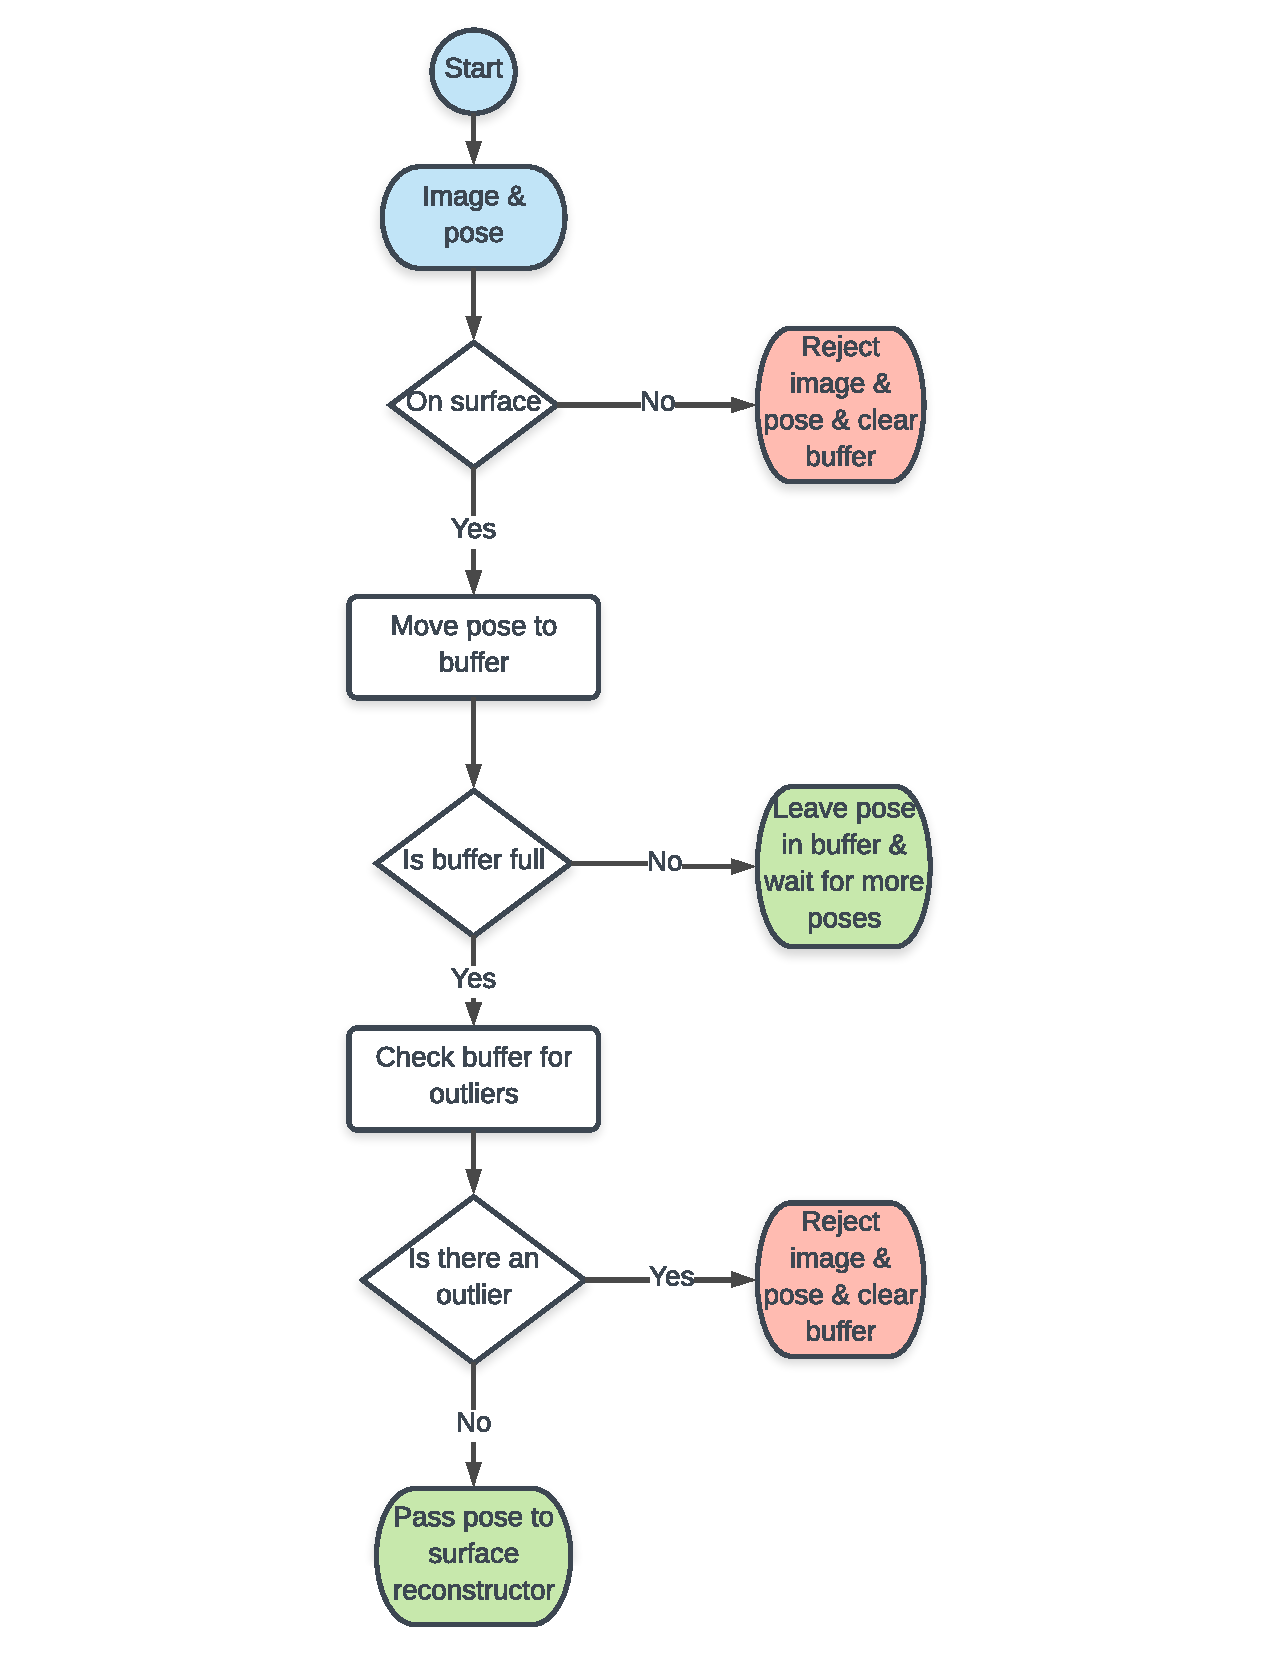
\includegraphics[width=0.65\textwidth]{SecondFlowChart}
  \caption{The way of the image and its pose if the surgeon is scanning the
    surface.}
  \label{fig:SecondFlowChart}
\end{figure}

\subsection{Surface contact detection}
For an image pose pair, the first step to pass is the contatct detection. Only
the ultrasound image is needed in this step. 

\begin{figure}[H]
  \centering
  \minipage{0.32\linewidth}
  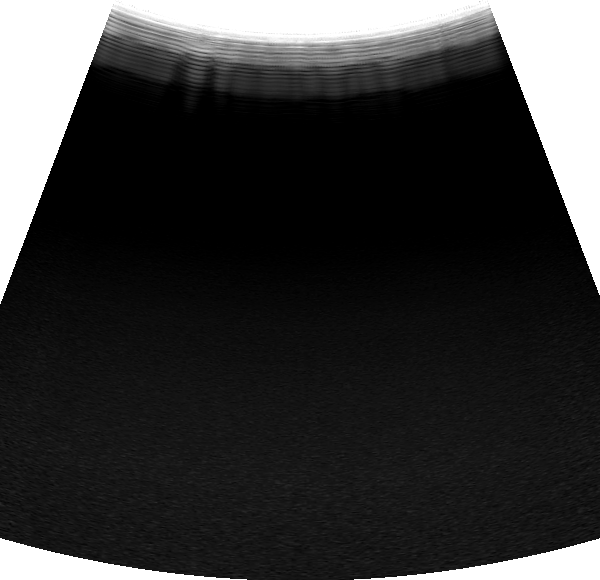
\includegraphics[width=\linewidth]{contact_no}
  \endminipage
  \hfill
  \minipage{0.32\linewidth}
  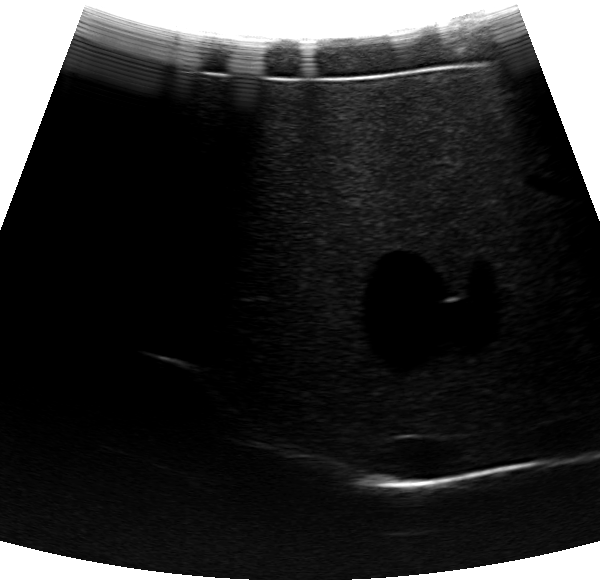
\includegraphics[width=\linewidth]{contact_difficult}
  \endminipage
  \hfill
  \minipage{0.32\linewidth}
  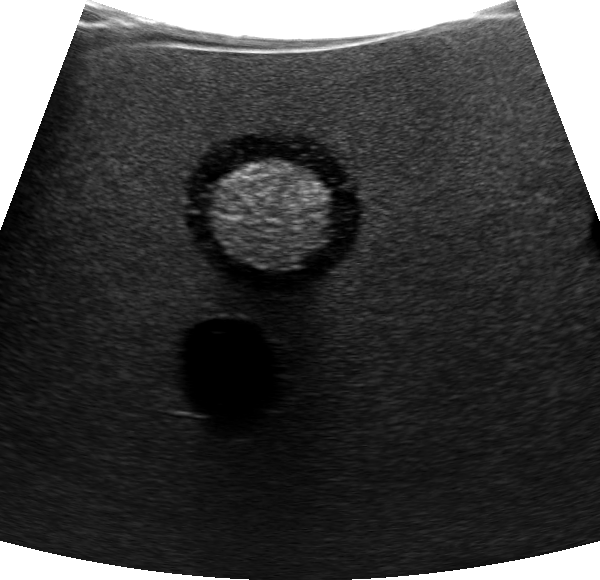
\includegraphics[width=\linewidth]{contact}
  \endminipage
  \hfill 
 \caption{Three ultrasound images from left to right: No contact with the liver,
   difficult to decide (In this case it would be contact because the middle part
   of the image shows contact), contact with the liver}
  \label{fig:contactVSnocontact}
\end{figure}

A classifier detects whether the US probe has contact to the liver or not. Therefore, a support vector machine (SVM) was trained with US images
from the phantom and from previous navigated liver surgeries. The SVM was trained to
classify the image into ``no surface contact'' (left) and ``surface contact'' (middle and right).
The images were labelled as "surface contact" if at least 50\% and the center had contact
to the surface (Figure 6.4 middle). The classifier takes into account that US waves are
reflected at the US probe-air interface when the US probe has no contact to the liver and
therefore no image is formed. The features for the classifier were: mean, median, minimum,
maximum, variance, skewness and kurtosis of the pixel values. All features are calculated
on the upper half of the image. For training, a set of 2'311 images (1'056 with contact, 1'255
without contact) were used. The training data was composed of images from a phantom
(88\%) and images from previous navigated liver surgeries (12\%). All computations were
performed using the SciPy software package. When the image is classified as ``surface contact'', then the position of the pose is stored
into the buffer. The buffer has a capacity of 10 positions. When
the addition of the actual pose leads to a full buffer, the buffer is
tested for outliers.
Each time a ``no surface contact'' image is classified and the positions buffer
is not empty it gets cleard.
\subsection{Outlier removal}
To find outliers in the current buffer the local
outlier factor is calculated for each position. 

\subsubsection{Local outlier factor}
The local outlier factor is a numerical value that describes the local density
of a position compared to its k-nearest neighbors (Figure
\ref{fig:lofExample}).

\begin{figure}[H]
  \centering
 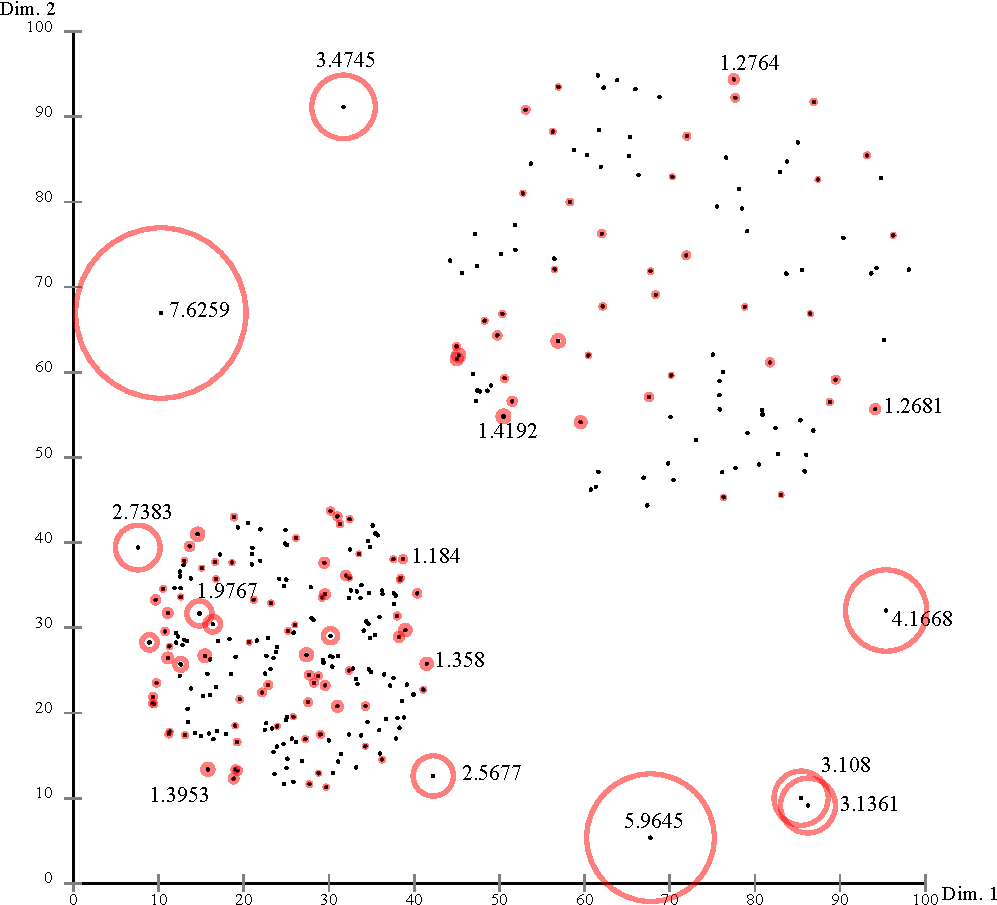
\includegraphics[width=0.8\textwidth]{lofExample}
  \caption{Example of the local outlier factors in a two dimensional pointcloud \cite{pictureLOF}.}
  \label{fig:lofExample}
\end{figure}

Five steps can be separeted to find the LOF of one position.
\begin{enumerate}
  \item{For each point calculate the distance to all the other points in the buffer}
  \item{For each point find the distance to his k-nearest neighbor $\rightarrow$
      \textit{k-distance}}
  \item{Find the \textit{reachability distance} from the k-nearest neighbors
      of each point to it self}
  \item{Calculate the \textit{local reachability density} for all points}
  \item{Calculate the \textit{local outlier factor}}
\end{enumerate}
The \textit{reachability distance} of point $A$ from another point $B$ is defined:
\begin{gather*}
  \mbox{reachability-d}_k(A,B)=\max\{\mbox{k\_d}(B), \mbox{d}(A,B)\}
\end{gather*}
The \textit{k-distance} of point $B$ depends on its k-nearest neighbors
and does not need to include point $A$.
But the actual distance between point $A$ and $B$ depends on only $A$
and $B$. The larger of the two will be the \textit{reachability distance} of
point $A$ from point $B$.

The \textit{local reachability density} of a point $A$ describes its neighborhood
and is defined by:
\begin{gather*}
  \mbox{LRD}(A):=1/\left(\frac{\sum_{B\in kNN(A)}\mbox{reachability-d}_k(A, B)}{|kNN(A)|}\right)
\end{gather*}
In words this is the inverse of the sum of the \textit{reachability distances} of point $A$
from its k-nearest neighbors devided by $k$.

Finally the \textit{local outlier factor} of a point $A$ indicates how his
neighborhood compares with the neighborhoods of his k-nearest neighbors. The LOF
of $A$ is defined by:
\begin{gather*}
  \mbox{LOF}(A):=\frac{\sum_{B\in kNN(A)}\frac{\mbox{LRD}(B)}{\mbox{LRD}(A)}}{|kNN(A)|}
\end{gather*}
If the neighborhood of $A$ is very similar to the neighborhoods of its k-nearest
neighbors, the LOF is close to 1. If its neighborhood is less dense than the
neighborhoods of his k-nearest neighbors, the LOF becomes larger than 1. If its
neighborhood is more dense than the neighborhoods of his k-nearest neighbors,
the LOF becomes lower than 1. \\
 \\
If an outlier is found in the buffer, the whole buffer is cleared. In the case
that no outlier is found, the oldest pose in the buffer gets moved into the
point collection to reconstruct the surface from.
\subsection{Reconstruction Parameters}
Finally there is a pointcloud with all the collected positions. This pointcloud
will be used as input for the surface reconstruction algorithm by Hoppe
\cite{hoppe1992surface}. The algorithm consists
of three phases. From an unorganized set of points, phase 1 constructs an
initial dense mesh. Starting with the dense mesh created in phase 1, phase 2
reduces the number of faces and improves the fit to the data points. In phase 3,
the surface representation is changed from a piecewise linear one (meshes) to a
piecewise smooth one. For the computations the implementation in VTK
(SurfaceReconstructionFilter) was used. The two main parameters of this
reconstruction algorithm have been optimized by applying the grid search method.
\subsubsection{Grid search for parameter optimization}
The \textit{neighborhood size} and the \textit{sample spacing} are the variable
parameters of the used surface reconstruction algorithm. The \textit{neighborhood size}
specifies the number of neighbors each point has. These neighbors are used to
estimate the local surface orientation. The \textit{sample spacing} sets the
spacing of a 3D sampling grid.
To find the optimal values to use in the algorithm with the point cloud data produced in the
experiment described in section \ref{sec:SurfaceReconstructionAccuracy}, a
first, rough grid search has been done to find the range of interest
of the two parameters. The same data was then used to do a second, more dense
grid search over the range of interest (Figure \ref{fig:gridSearchResultMean} and
\ref{fig:gridSearchResultSTD}). For each parameter setting, the average distance from the
reference points to the reconstructed surface was calculated.
\begin{figure}[h]
  \centering
 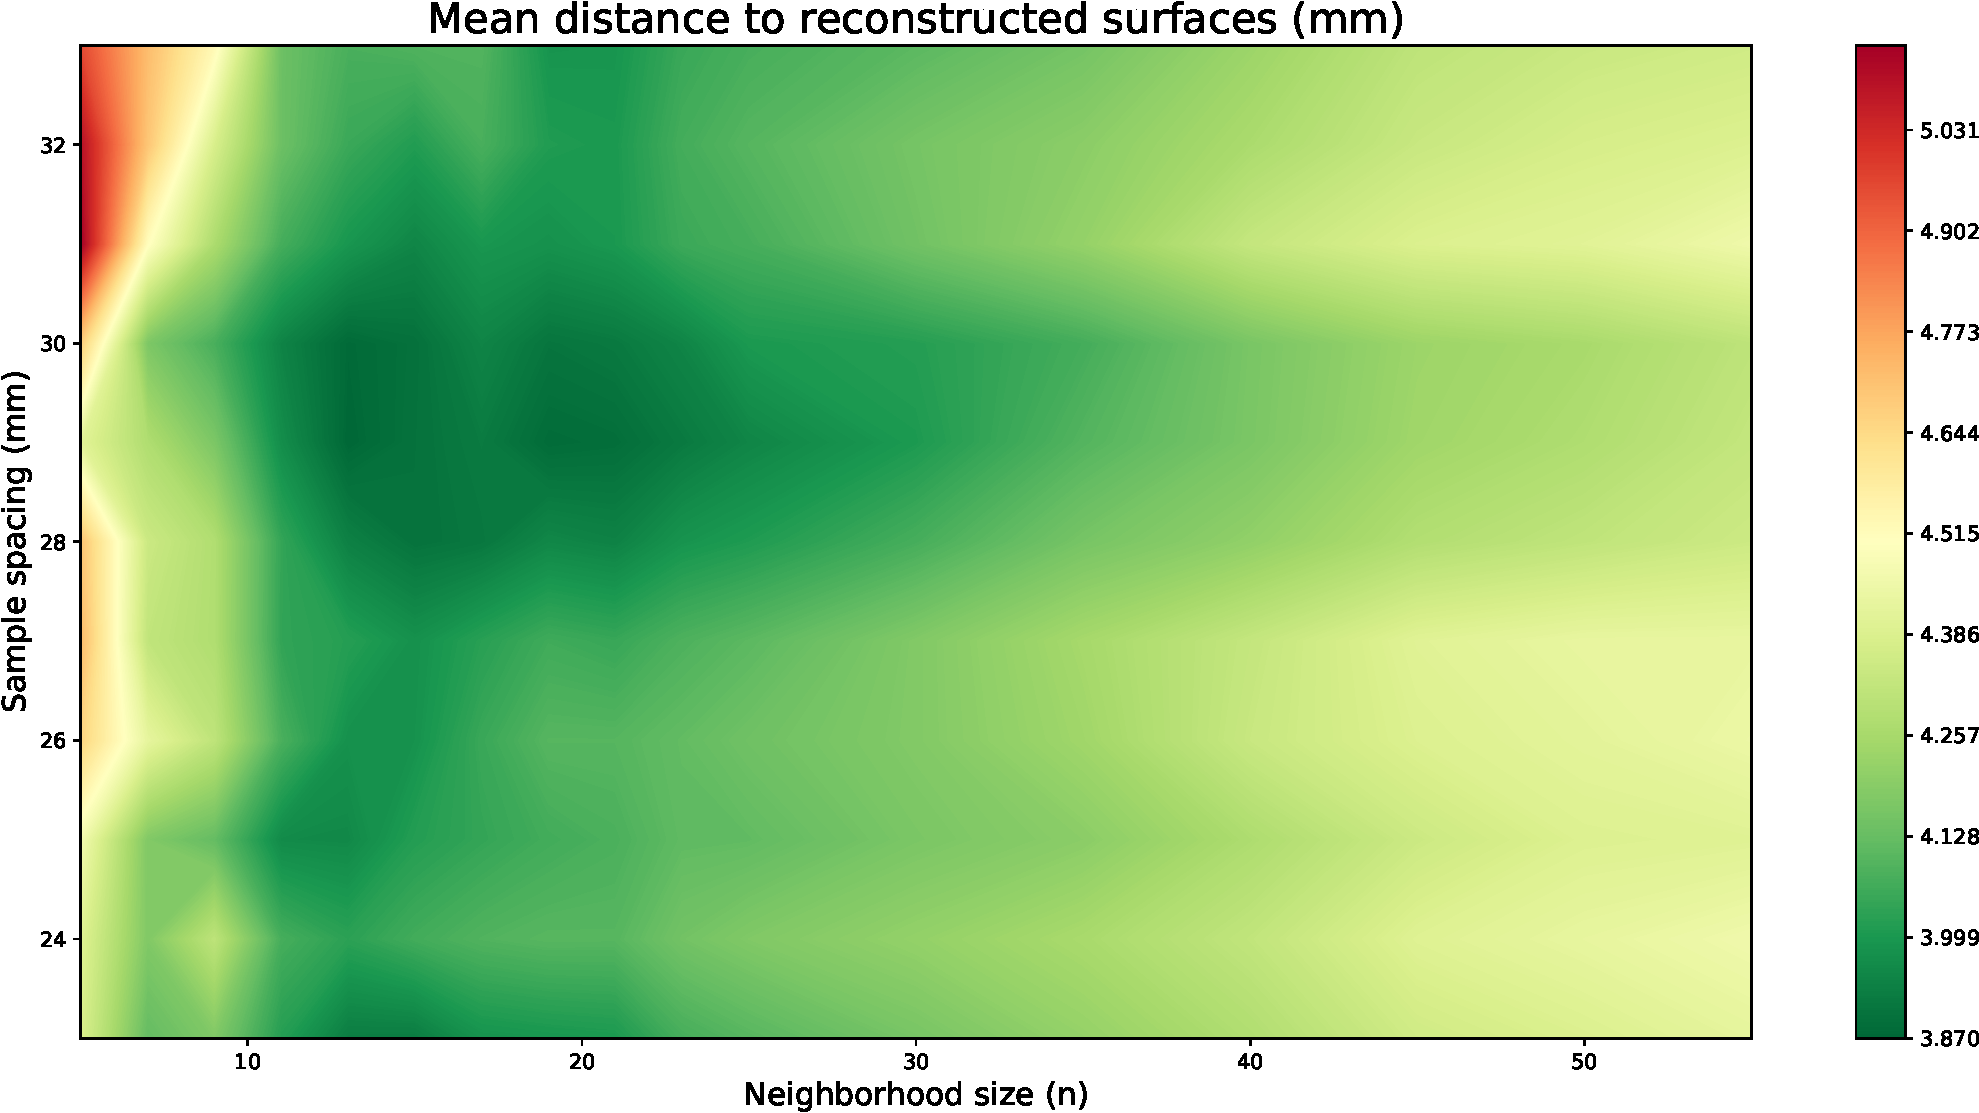
\includegraphics[width=0.9\textwidth]{gridSearchResultMeanCrop}
  \caption{This contour plot shows the mean distance calculated over 10
    differently sampled point collections. All point collections represent the
    surface of the same liver phantom.}
  \label{fig:gridSearchResultMean}
\end{figure}
The found mean distance varies from 5.1 mm to 3.9 mm. Neighborhood sizes smaller
than 8 show an increase of the mean distance for sample spacings larger than 25
mm. Neighborhood sizes over 30 seem to increase the mean distance also.
The standard deviation of the mean varies between 6.1 mm and 4.6 mm. These high
deviations result mostly from the boarder part of the reconstructions where the
reference points are more than 2 cm away from the surfaces (see section
\ref{sec:SurfaceReconstructionAccuracy}). One can say the standard deviation of
the mean decreases together with the neighborhood size used for the
reconstruction. But this is only true for neighborhood sizes larger than 13.
Because from neighborhood size 13 till 10 the standard deviation increases not
till then it decreases again. 

\begin{figure}[h]
  \centering
 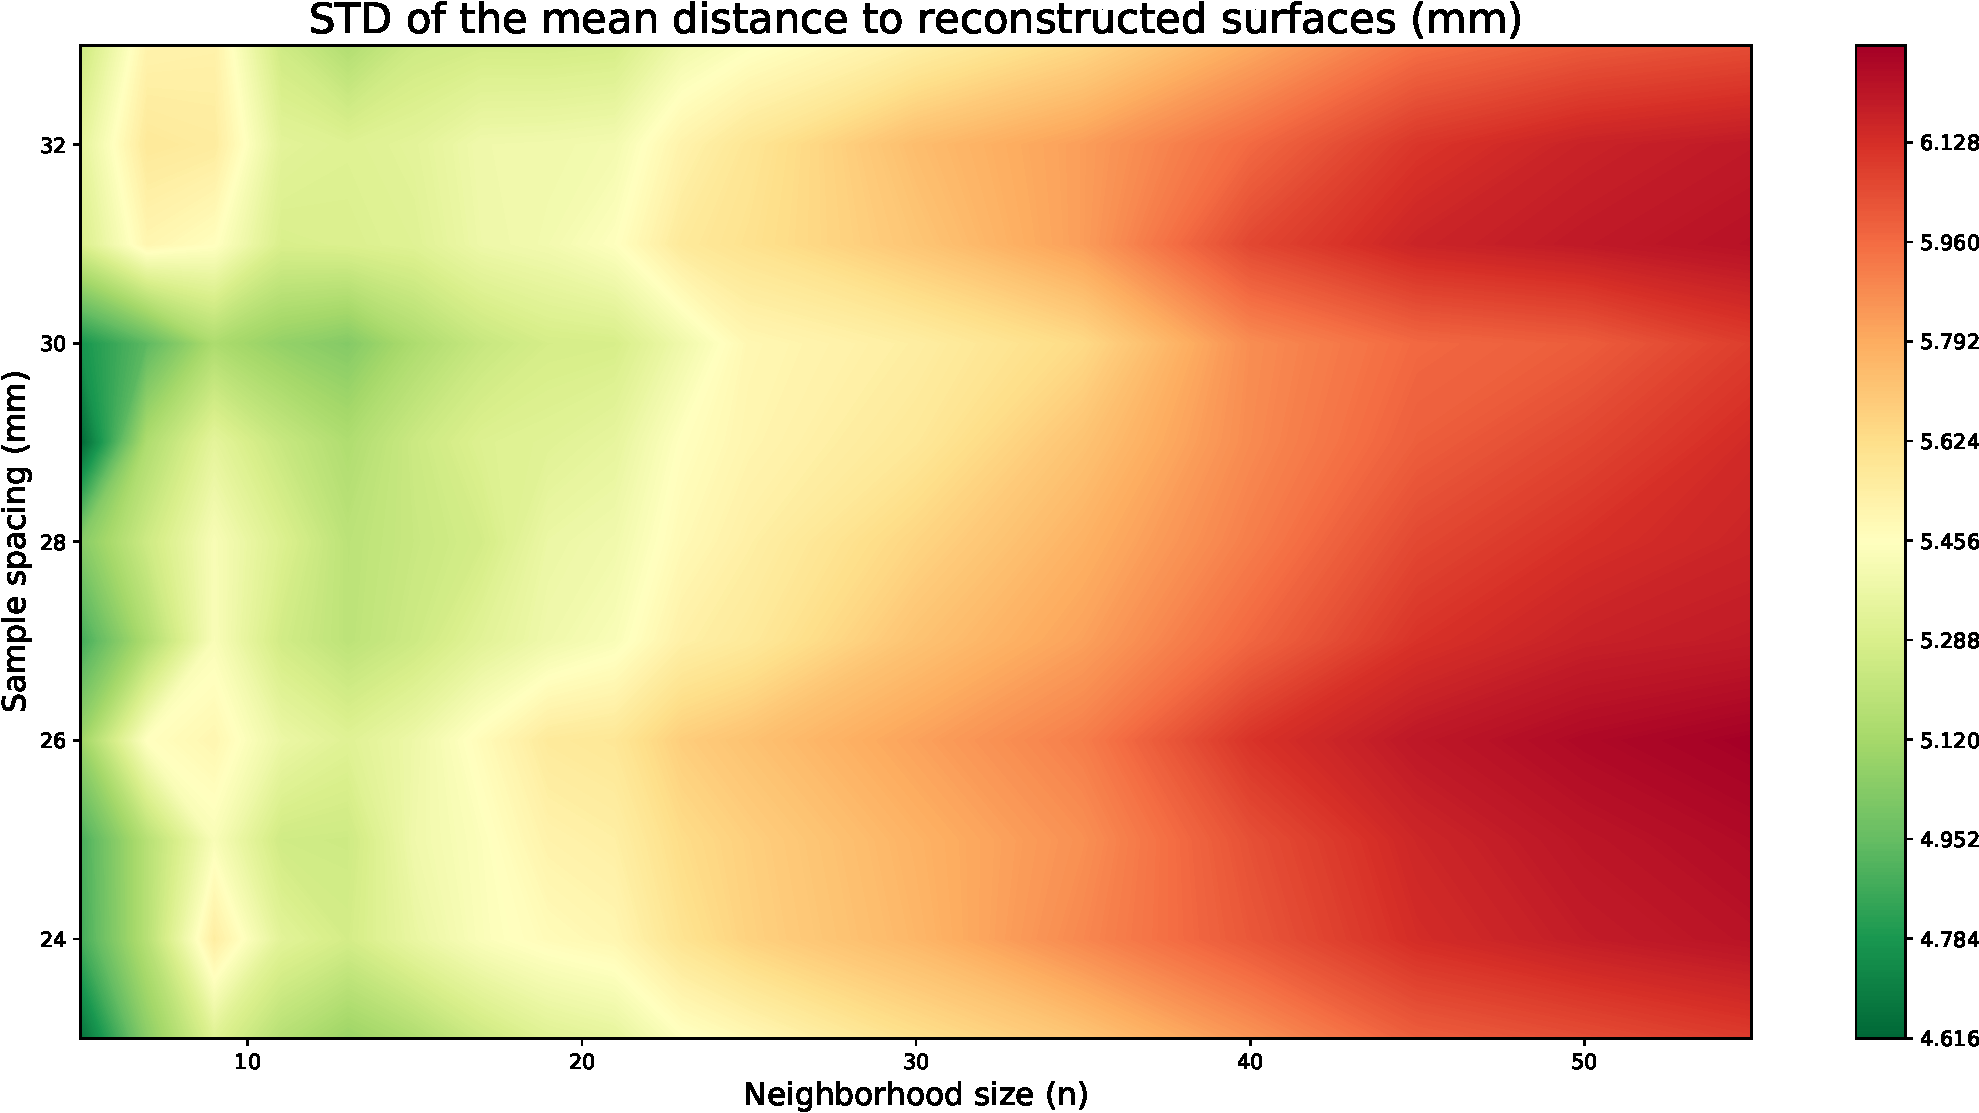
\includegraphics[width=0.9\textwidth]{gridSearchResultSTDCrop}
  \caption{This contour plot shows the STD of the mean distance calculated over 10
    differently sampled point collections. All point collections represent the
    surface of the same liver phantom.}
  \label{fig:gridSearchResultSTD}
\end{figure}

By simply summing up the mean and the standard deviation, one finds that the
optimal parameters for the tested surface samplings are 13 for the neighborhood
size and 30 mm for the sample spacing.


grid search
\section{Tumor Segmentation}

\begin{figure}[H]
  \centering
 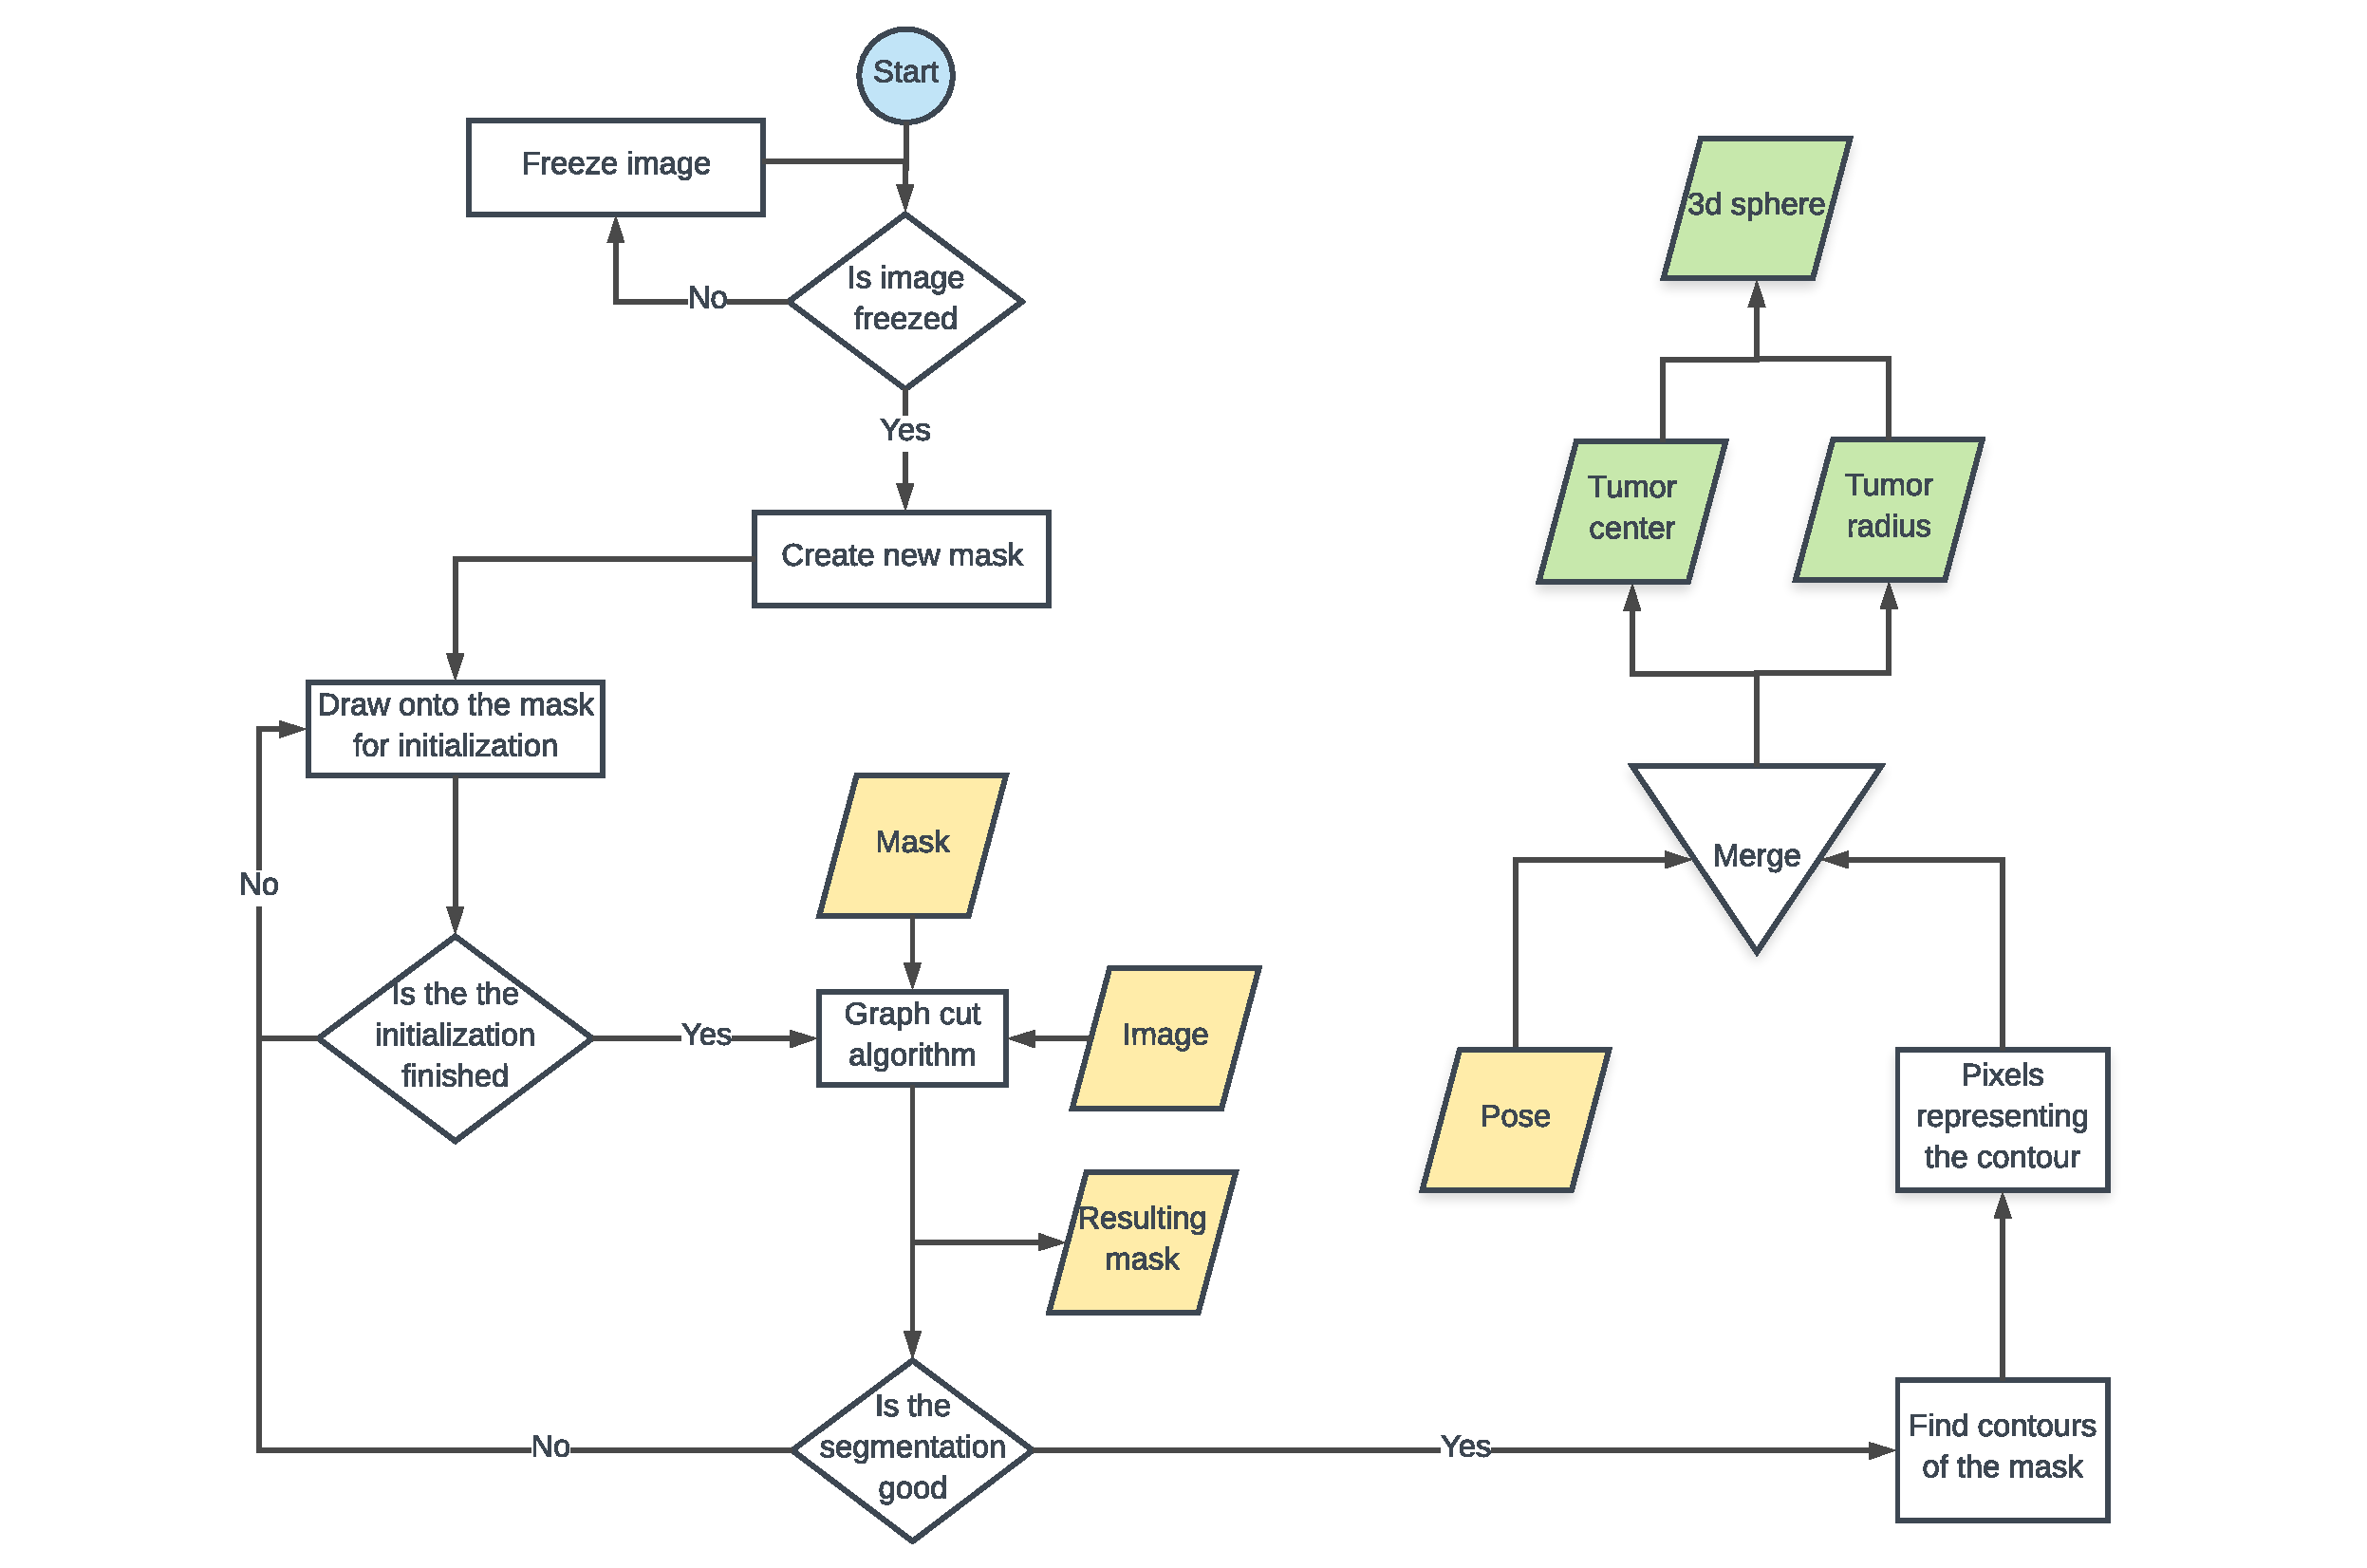
\includegraphics[width=1.2\textwidth]{ThirdFlowChart}
  \caption{The way of the image and its pose if the surgeon is scanning the
    surface.}
  \label{fig:ThirdFlowChart}
\end{figure}

graph cuts
initialization method
\section{Resection Planning}
\subsection{Cone fitting around tumor}
\section{Visualization for navigation}
\subsection{Ultrasound overlay}
The ultrasound image ...
\begin{figure}[H]
  \centering
  \minipage{0.48\linewidth}
  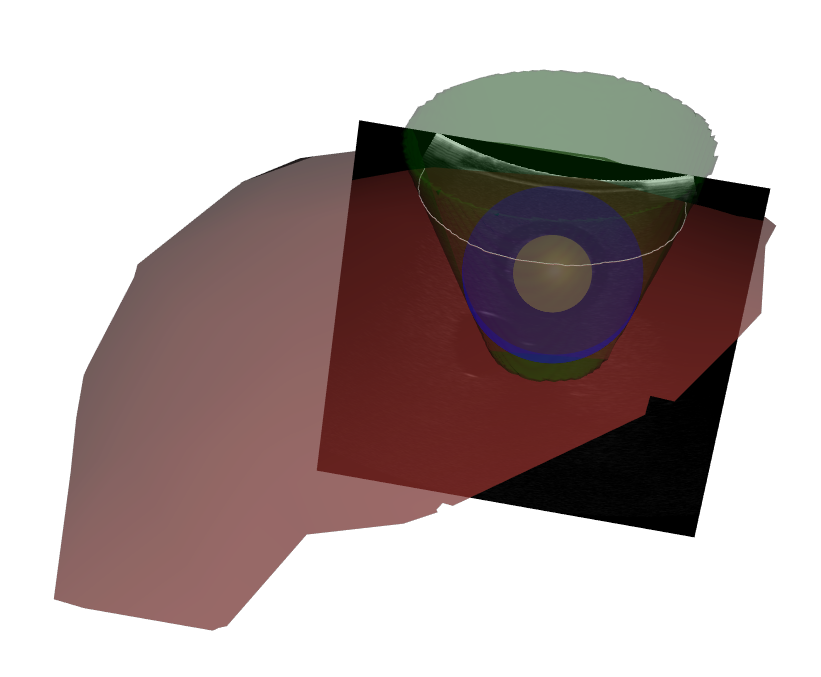
\includegraphics[width=\linewidth]{cutter3DView} 
  \endminipage
  \hfill
  \minipage{0.48\linewidth}
  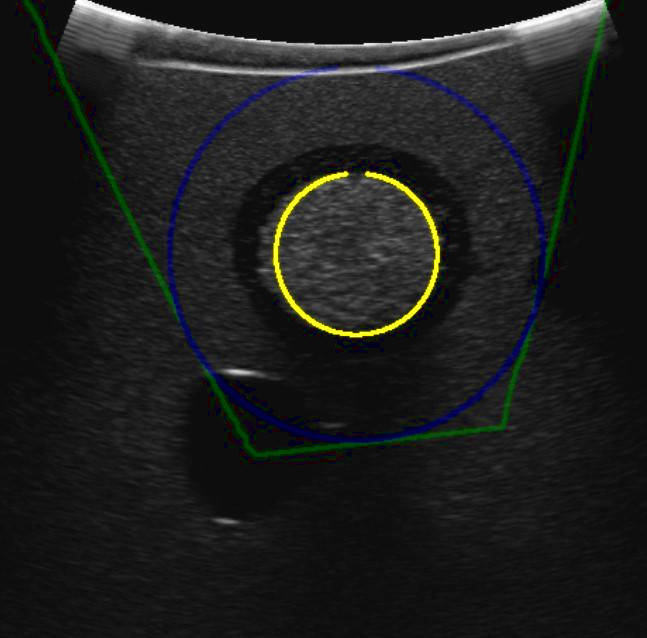
\includegraphics[width=\linewidth]{cutter2DView}
  \endminipage
  \hfill 
 \caption{On the left side is the 3D scene with the ultrasound image cutting
   through the tumor, safety margin and the resection plane. On the right side
   is the resulting cutting overlay on the live ultrasound image.}
  \label{fig:cutterExample}
\end{figure}
\subsection{3D model}
\section{UI Concept}
%%% Local Variables:
%%% TeX-master: "MscThesis"
%%% End: